
\documentclass[border=8pt, multi, tikz]{standalone} 
\usepackage[fontsize=14pt]{fontsize}
\usepackage{import}
\subimport{../layers/}{init}
\usetikzlibrary{positioning}
\usetikzlibrary{3d} %for including external image 

\def\ConvColor{rgb:yellow,5;red,2.5;white,5}
\def\ConvReluColor{rgb:yellow,5;red,5;white,5}
\def\PoolColor{rgb:red,1;black,0.3}
\def\UnpoolColor{rgb:blue,2;green,1;black,0.3}
\def\FcColor{rgb:blue,5;red,2.5;white,5}
\def\FcReluColor{rgb:blue,5;red,5;white,4}
\def\SoftmaxColor{rgb:magenta,5;black,7}   
\def\SumColor{rgb:blue,5;green,15}

\newcommand{\copymidarrow}{\tikz \draw[-Stealth,line width=0.8mm,draw={rgb:blue,4;red,1;green,1;black,3}] (-0.3,0) -- ++(0.3,0);}
\begin{document}
\begin{tikzpicture}
\tikzstyle{connection}=[ultra thick,every node/.style={sloped,allow upside down},draw=\edgecolor,opacity=0.7]
\tikzstyle{copyconnection}=[ultra thick,every node/.style={sloped,allow upside down},draw={rgb:blue,4;red,1;green,1;black,3},opacity=0.7]

\node[canvas is zy plane at x=0] (map) at (-2.5,0,0) {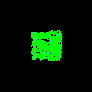
\includegraphics[width=6.0cm,height=6.0cm]{internal_map.png}};

\pic[shift={(0,0,0)}] at (0,0,0) 
    {Box={
        name=input,
        caption=$\tilde{Z}_t$,
        xlabel={{3, }},
        zlabel=60,
        fill=\FcColor,
        height=30.0,
        width=0.375,
        depth=30.0
        }
    };

\pic[shift={(2.75,0,0)}] at (input-east) 
    {Box={
        name=conv1,
        caption= ,
        xlabel={{32, }},
        zlabel=56,
        fill=\ConvColor,
        height=28.0,
        width=4.0,
        depth=28.0
        }
    };

\draw [connection]  (input-east)    -- node {\midarrow} (conv1-west);

\pic[shift={ (0,0,0) }] at (conv1-east) 
    {Box={
        name=pool1,
        caption= ,
        fill=\PoolColor,
        opacity=0.5,
        height=14.0,
        width=4.0,
        depth=14.0
        }
    };

\pic[shift={(1.5625,0,0)}] at (pool1-east) 
    {Box={
        name=conv2,
        caption= ,
        xlabel={{64, }},
        zlabel=24,
        fill=\ConvColor,
        height=12.0,
        width=8.0,
        depth=12.0
        }
    };

\draw [connection]  (pool1-east)    -- node {\midarrow} (conv2-west);

\pic[shift={ (0,0,0) }] at (conv2-east) 
    {Box={
        name=pool2,
        caption= ,
        fill=\PoolColor,
        opacity=0.5,
        height=6.0,
        width=8.0,
        depth=6.0
        }
    };

\pic[shift={(1.0,0,0)}] at (pool2-east) 
    {Box={
        name=conv3,
        caption= ,
        xlabel={{64, }},
        zlabel=8,
        fill=\ConvColor,
        height=4.0,
        width=8.0,
        depth=4.0
        }
    };

\draw [connection]  (pool2-east)    -- node {\midarrow} (conv3-west);

\pic[shift={ (0,0,0) }] at (conv3-east) 
    {Box={
        name=pool3,
        caption= ,
        fill=\PoolColor,
        opacity=0.5,
        height=2.0,
        width=8.0,
        depth=2.0
        }
    };

\pic[shift={(1.25,0,0)}] at (pool3-east) 
    {Ball={
        name=sum1,
        fill=\SumColor,
        opacity=0.6,
        radius=2,
        logo=$+$
        }
    };

\pic[shift={(-1,3,0)}] at (sum1-east) 
    {Box={
        name=obs,
        caption=$O_t$\newline,
        xlabel={{, }},
        zlabel=4,
        fill=\FcColor,
        height=1,
        width=1,
        depth=3.0
        }
    };

\draw [connection]  (pool3-east)    -- node {\midarrow} (sum1-west);

\draw [connection]  (obs-east)    -- node {\midarrow} (sum1-west);

\pic[shift={(1.125,0,0)}] at (sum1-east) 
    {Box={
        name=soft1,
        caption= ,
        xlabel={{" ","dummy"}},
        zlabel=256,
        fill=\SoftmaxColor,
        opacity=0.8,
        height=1,
        width=1,
        depth=96.0
        }
    };

\draw [connection]  (sum1-east)    -- node {\midarrow} (soft1-west);

\pic[shift={(1.25,0,0)}] at (soft1-east) 
    {Ball={
        name=sum2,
        fill=\SumColor,
        opacity=0.6,
        radius=2,
        logo=$+$
        }
    };

\pic[shift={(1,2,0)}] at (sum2-east) 
    {Box={
        name=action,
        caption=$A_t$,
        xlabel={{, }},
        zlabel=1,
        fill=\FcColor,
        height=1,
        width=1,
        depth=0.75
        }
    };

\draw [connection]  (action-east)    -- node {\midarrow} (sum2-west);

\draw [connection]  (soft1-east)    -- node {\midarrow} (sum2-west);

\pic[shift={(1.125,0,0)}] at (sum2-east) 
    {Box={
        name=soft2,
        caption= ,
        xlabel={{" ","dummy"}},
        zlabel=128,
        fill=\SoftmaxColor,
        opacity=0.8,
        height=1,
        width=1,
        depth=48.0
        }
    };

\draw [connection]  (sum2-east)    -- node {\midarrow} (soft2-west);

\pic[shift={(1.125,0,0)}] at (soft2-east) 
    {Box={
        name=soft3,
        caption= ,
        xlabel={{" ","dummy"}},
        zlabel=64,
        fill=\SoftmaxColor,
        opacity=0.8,
        height=1,
        width=1,
        depth=24.0
        }
    };

\draw [connection]  (soft2-east)    -- node {\midarrow} (soft3-west);

\pic[shift={(1.125,0,0)}] at (soft3-east) 
    {Box={
        name=output,
        caption=Output $\hat{q}_{\mathbf{\phi}}({Z_t,A_t})$,
        xlabel={{" ","dummy"}},
        zlabel=1,
        fill=\SoftmaxColor,
        opacity=0.8,
        height=1,
        width=1,
        depth=1.5
        }
    };

\draw [connection]  (soft3-east)    -- node {\midarrow} (output-west);

\pic[shift={(-8.5,-4)}] at (output-east) 
    {Box={
        name=input_legend,
        caption=Input,
        xlabel={{, }},
        zlabel=,
        fill=\FcColor,
        height=1,
        width=1,
        depth=1
        }
    };

\pic[shift={(-6.5,-4)}] at (output-east) 
    {Box={
        name=conv_legend,
        caption=Conv 5x5 + ReLU,
        xlabel={{, }},
        zlabel=,
        fill=\ConvColor,
        height=1,
        width=1,
        depth=1
        }
    };

\pic[shift={ (-4.5,-4) }] at (output-east) 
    {Box={
        name=pool_legend,
        caption=Max-Pool 2x2,
        fill=\PoolColor,
        opacity=0.5,
        height=1,
        width=1,
        depth=1
        }
    };

\pic[shift={(-2.5,-4)}] at (output-east) 
    {Box={
        name=soft_legend,
        caption=FC + ReLU,
        xlabel={{" ","dummy"}},
        zlabel=,
        fill=\SoftmaxColor,
        opacity=0.8,
        height=1,
        width=1,
        depth=1
        }
    };

\pic[shift={(-1.1,-4)}] at (output-east) 
    {Box={
        name=sum_legend_caption,
        caption=Concate-nation,
        xlabel={{" ","dummy"}},
        zlabel=,
        fill=\SoftmaxColor,
        opacity=0.8,
        height=0,
        width=0,
        depth=0
        }
    };

\pic[shift={(0,-4)}] at (output-east) 
    {Ball={
        name=sum_legend,
        fill=\SumColor,
        opacity=0.6,
        radius=1,
        logo=$+$
        }
    };

\end{tikzpicture}
\end{document}
